\documentclass[11pt,a4paper]{article}
\usepackage[margin=2.4cm]{geometry}
\usepackage[utf8]{inputenc}
\usepackage[T1]{fontenc}
\usepackage{lmodern}
\usepackage{microtype}
\usepackage{amsmath,amssymb}
\usepackage{booktabs,tabularx,array}
\usepackage{enumitem}
\usepackage{caption}
\usepackage{xcolor}
\usepackage{pgfplots}
\pgfplotsset{compat=1.17}
\usepackage[hidelinks]{hyperref}
\setlist{itemsep=1pt,topsep=3pt}
\setlength{\emergencystretch}{2em}
\captionsetup{font=small}

% Numbers: experiments/gpdp/results/{report_evaluate,relative_errors_report,check1_evaluate,
% relative_errors,relative_errors_rspg_blocks}.json; runs/endogenous/gpdp/report_singlevgp_a1_s*/log.json.
% Reproduce the GPDP runs with experiments/gpdp/run_report_config.sh.

\title{Gaussian-process dynamic programming for a heterogeneous-agent mean-field game\\
\large An alternative to recurrent structural policy gradient in MFAX}
\author{[Your name]}
\date{October 14, 2026}

\begin{document}
\maketitle

%=====================================================================
\section{Introduction}

Heterogeneous-agent economies, with many households that save, consume and interact through prices,
are \emph{mean-field games}: each household is too small to move prices, but the distribution of all
households determines them. An equilibrium is a decision rule that is optimal for every household,
given the prices that the whole population generates by following it.

Wibault et al.~\cite{rspg} solve such games with \emph{recurrent structural policy gradient} (RSPG),
implemented in the MFAX library and building on structural policy gradient~\cite{spg}. RSPG learns
the households' decision rule with a neural network trained by gradient descent.

This report presents a different way to obtain the decision rule, adapted from
\emph{Gaussian-process dynamic programming} (GPDP)~\cite{deisenroth}. Instead of improving a network
step by step, GPDP computes the best decisions directly, by dynamic programming backward in time,
and uses two Gaussian processes (GPs): one to value the future state of the economy, and one to
represent the decision rule. We describe the algorithm and compare it with RSPG on MFAX's
macroeconomic model.

%=====================================================================
\section{The model}\label{sec:model}

We use MFAX's \emph{endogenous} model, a heterogeneous-agent economy in the style of
Aiyagari~\cite{aiyagari} and Krusell--Smith~\cite{ks}.
\begin{itemize}
\item \textbf{Households.} A household's state is $s = (b, y)$: wealth $b$ (a 200-point grid) and
  income $y$ (5 levels, moving randomly up or down). There are $|\mathcal S| = 1000$ individual states.
\item \textbf{Decision.} A household with cash on hand $B_t(s) = (1+r_t)\,b + w_t\,y$ consumes a
  share $a \in (0,1)$ of it and saves the rest. Utility is $u(c) = c^{1-\sigma}/(1-\sigma)$ with
  $\sigma = 2$, and the discount factor is $\gamma = 0.95$.
\item \textbf{Prices.} The interest rate $r_t$ and the wage $w_t$ follow from a Cobb--Douglas
  technology. They depend on aggregate capital $K_t$ (average wealth) and a productivity shock $z_t$,
  common to all households, with $z_{t+1} = 0.9\,z_t + 0.03\,\varepsilon_{t+1}$,
  $\varepsilon_{t+1} \sim \mathcal N(0,1)$.
\item \textbf{Horizon.} An episode lasts $T = 128$ periods, from a uniform distribution and $z_0 = 0$.
  In the last period households consume all their cash on hand.
\end{itemize}
The state of the economy is the distribution $\mu_t$ of households over $\mathcal S$ (a vector of
1000 shares) together with $z_t$. Because average income is constant in this model, the two observed
prices reveal $(z_t, K_t)$ exactly: households effectively observe $(z_t, K_t)$.

%=====================================================================
\section{RSPG in brief}

RSPG represents the decision rule by a neural network. Its inputs are the household's state and a
summary of past prices produced by a recurrent network; its output is a probability for each of 20
consumption shares $\{0.025, 0.075, \ldots, 0.975\}$. One training step simulates 8 economies over
the whole episode, computes the value of every household state exactly by backward recursion, and
moves the network's weights in the direction that raises these values (prices held fixed). Training
takes 500 such steps; most of the cost is simulating and differentiating through 128 periods at
every step.

%=====================================================================
\section{GPDP in brief}

Dynamic programming finds the best decision backward in time: the value of a state today is the best,
over actions, of today's utility plus the discounted value of where the action leads tomorrow.
Starting from the known value at the end, it moves back one period at a time.

GPDP~\cite{deisenroth} extends this to states that cannot be enumerated: values are computed exactly
at a few sampled states and a GP fills them in elsewhere; a second GP, fitted on the best actions,
gives the decision rule. In our game:
\begin{itemize}
\item \textbf{a household's own problem is small and known exactly} (1000 states, known transitions,
  one decision), so best decisions are computed exactly by a one-dimensional search, with any share
  in $(0,1)$ allowed;
\item \textbf{the state of the economy is what cannot be enumerated}, so the GPs only have to learn how
  values and decisions depend on the economy and on time.
\end{itemize}
The households' decision rule is thus obtained without gradient descent and without a neural
network.\footnote{The GPs' hyperparameters are still fitted by gradient-based maximization of the
marginal likelihood.}

%=====================================================================
\section{Implementation}\label{sec:impl}

\subsection{The algorithm}
\begin{center}
\fbox{\begin{minipage}{0.93\linewidth}
\textbf{Start:} every household consumes 15\% of its cash on hand, whatever its state, the
economy or the date.\\[2pt]
\textbf{Repeat} (one \emph{iteration}):
\begin{enumerate}
\item \textbf{Forward pass:} simulate $N = 8$ economies for 128 periods under the current decision
  rule, and store their states (Section~\ref{sec:forward}).
\item \textbf{Backward pass:} from the last period to the first, compute the best share and its value
  for every household state in every simulated economy, and train the value GP on these values
  (Section~\ref{sec:backward}).
\item \textbf{Policy fit:} fit the policy GP on the best shares. It becomes the households' decision
  rule for the next iteration.
\end{enumerate}
\end{minipage}}
\end{center}
The 15\% start contains no information about the equilibrium (it ignores wealth, income, prices and
time) but is economically plausible (trained policies consume 11--19\% of cash on hand on average).
The population adopts the new decision rule in full at each iteration.

\subsection{Forward pass: what is simulated and stored}\label{sec:forward}
Each simulated economy $n = 1,\ldots,8$ starts from the uniform distribution and $z_0 = 0$. At each
period $t$:
\begin{enumerate}
\item the households' shares come from the current decision rule, evaluated at the economy's
  $(z_t, K_t)$ and the time left $\tau = T - t$;
\item the distribution moves forward exactly: each state's mass consumes its share, saves the rest,
  and is spread over next period's wealth grid points and income levels with the known transition
  probabilities;
\item a new shock $z_{t+1}$ is drawn, and the new prices follow.
\end{enumerate}
We store, for every economy and period, the distribution $\mu_t^n$, the shock $z_t^n$, capital
$K_t^n$ and the prices. These $8 \times 128$ economy states are the \emph{support points} at which the
backward pass computes exact values. The full distribution $\mu_t^n$ is needed for two things: it
gives today's prices, and it gives tomorrow's capital $K_{t+1}^n$, which depends on today's
decisions but not on tomorrow's shock.

\subsection{Backward pass}\label{sec:backward}
\paragraph{Last period.} At $t = 127$ households consume everything, so the value is known exactly:
$V_{127}(s) = u\big(B_{127}(s)\big)$, for any $(z, K)$.

\paragraph{Earlier periods, $t = 126, \ldots, 0$.} For each simulated economy $n$:
\begin{enumerate}
\item \textbf{Tomorrow's values, averaged over tomorrow's shock.} Tomorrow's capital $K_{t+1}^n$ is
  known; tomorrow's shock is not. We take 5 possible values $z'_q = 0.9\,z_t^n + 0.03\,\epsilon_q$
  with probabilities $w_q$ (Gauss--Hermite quadrature) and ask the value GP for tomorrow's values
  there:
  \[
  W(s') \;=\; \sum_{q=1}^{5} w_q\, \widehat V\big(s';\, z'_q,\, K_{t+1}^n,\, \tau-1\big)
  \qquad \text{for every } s' \in \mathcal S .
  \]
  Averaging \emph{before} choosing matters: choosing with the shock that actually occurred would use
  information households do not have.
\item \textbf{Best share for every household state.} For each $s \in \mathcal S$,
  \[
  a^*_t(s) = \arg\max_{a \in (0,1)} Q_t(s,a), \qquad
  Q_t(s,a) = u\big(a\,B_t(s)\big) + \gamma \sum_{s'} P_t(s' \mid s,a)\, W(s'),
  \]
  where $P_t(s'\mid s,a)$ is the known probability of moving to state $s'$ (next wealth
  $(1-a)B_t(s)$ spread over its two neighbouring grid points, times the income transition). The
  maximum is found by golden-section search (30 steps, precision about $10^{-4}$), and
  $V_t(s) = Q_t\big(s, a^*_t(s)\big)$.
\item \textbf{Training data.} The 1000 values $V_t(\cdot)$ at economy $n$ are added to the value GP's
  training set, and the value GP is refitted before moving to period $t-1$.
\end{enumerate}
At the end of the backward pass we have, for every economy and every period, the best share of every
household state: the training targets of the policy GP.

\subsection{The two Gaussian processes}
Both GPs map a few numbers describing the economy to a vector of 1000 numbers, one per household
state. The household's own state is therefore not an input: it indexes the outputs.

\begin{table}[h]
\centering
\small
\renewcommand{\arraystretch}{1.25}
\begin{tabularx}{\linewidth}{@{}>{\raggedright\arraybackslash}p{2.3cm}>{\raggedright\arraybackslash}X>{\raggedright\arraybackslash}X@{}}
\toprule
 & \textbf{Value GP} $\widehat V$ & \textbf{Policy GP} $\widehat \pi$ \\
\midrule
Input & $x = (z, K, \tau) \in \mathbb R \times \mathbb R_{>0} \times \{1,\ldots,128\}$ \newline
        shock, capital, time left & same: $x = (z, K, \tau)$ \\
Output & a vector in $\mathbb R^{1000}$: for each $s$, $\log \bar c(s)$, the log of the constant
         consumption with the same value (below) & a vector in $\mathbb R^{1000}$: for each $s$, the
         log-odds $\ell(s) = \log\frac{a(s)}{1-a(s)}$ of the consumption share \\
Returned to the algorithm & values $V(s) = D(\tau)\, u\big(\bar c(s)\big)$ &
         shares $a(s) = 1/(1+e^{-\ell(s)}) \in (0,1)$ \\
Fitted on & the values $V_t(s)$ computed in the backward pass, at every simulated economy and solved
            period: up to $8 \times 126 = 1008$ inputs, each with 1000 targets &
            the best shares $a^*_t(s)$, at every simulated economy and decision period:
            $8 \times 127 = 1016$ inputs, each with 1000 targets \\
Fitted when & during the backward pass: period $t$ uses the GP fitted on periods $t+1,\ldots,126$ &
              once per iteration, after the backward pass \\
Used for & tomorrow's values in the backward pass & the households' decisions in the next forward
           pass and in the evaluation \\
\bottomrule
\end{tabularx}
\end{table}

\paragraph{Why these inputs.} Prices depend only on $(z, K)$, and households observe them through
prices. Krusell and Smith~\cite{ks} showed that such a summary of the distribution is enough to
forecast prices accurately in this class of economies. The time left $\tau$ is needed because the
horizon is finite: values shrink and households spend their savings as the end approaches.

\paragraph{Why the value GP predicts $\log \bar c$.} Lifetime values grow about twentyfold from the
last period to the first, simply because more periods remain. Writing $V = D(\tau)\,u(\bar c)$, with
$D(\tau) = \sum_{j=0}^{\tau-1}\gamma^j$ the weight of the remaining periods, removes that trend: the
constant-consumption equivalent $\bar c$ changes little over the episode, and is what the GP learns.

\paragraph{Kernel.} Both GPs use one squared-exponential kernel with a length scale per input,
shared by all 1000 outputs:
\[
k(x, x') \;=\; s_f^2 \exp\Big(-\tfrac12 \sum_{d=1}^{3} \frac{(x_d - x'_d)^2}{\ell_d^2}\Big)
\;+\; s_n^2\, \mathbb 1[x = x'] ,
\]
on standardized inputs and outputs. Economies with similar shock, capital and time left get similar
values and decisions; the length scales $\ell_d$ say how quickly this similarity fades along each
input. The hyperparameters $(\ell_d, s_f, s_n)$ maximize the marginal likelihood, within bounds that
keep the computations numerically stable. Since all outputs share the kernel, a single matrix
factorization serves all 1000 of them.

\paragraph{Evaluation on MFAX's actions.} MFAX evaluates policies over its 20 shares. For that
evaluation only, each GPDP share is replaced by the nearest of the 20.

%=====================================================================
\section{Metrics}\label{sec:metrics}

\paragraph{Exploitability.} How much a single household could gain by changing its decisions while
everyone else keeps the population's rule $\pi$. With $m^{\pi,\omega}$ the path of the economy
generated by $\pi$ under the shocks $\omega$, and $V^{\pi'}_0(s\mid m)$ the expected discounted
utility of a household starting in $s$ and following $\pi'$ along that path,
\[
\mathcal E(\pi) \;=\; \mathbb E_\omega \sum_{s} \mu_0(s)\Big[\max_{\pi'} V^{\pi'}_0\big(s\mid m^{\pi,\omega}\big)
- V^{\pi}_0\big(s\mid m^{\pi,\omega}\big)\Big].
\]
The maximizing $\pi'$ is the \emph{best response}. Exploitability is zero exactly at an equilibrium.
We report it as computed by MFAX (best response over the 20 shares, computed on each realized path),
and in consumption units against a best response allowed any share (next paragraph).

\paragraph{Consumption-equivalent (CE) relative error.} Values are in utility units, which are hard
to read, and ratios of values explode near zero. We therefore express a value $V$ as the constant
consumption $\bar c$ giving the same lifetime utility. The relative error of the policy's value with
respect to the best response's, for household state $s$, is
\[
\varepsilon(s) \;=\; \frac{\bar c_{\pi}(s) - \bar c_{\mathrm{BR}}(s)}{\bar c_{\mathrm{BR}}(s)}
\;=\; \left(\frac{V_\pi(s)}{V_{\mathrm{BR}}(s)}\right)^{1/(1-\sigma)} - 1 .
\]
$|\varepsilon(s)| = 1\%$ means: following the population's rule is worth as much as consuming 1\%
less, every period, than with the best response. We report its average over households, weighted by
where they are: at the start of the episode (the weighting of exploitability), and over all periods
(the value of the remaining lifetime at each period). The \emph{gain from deviating} applies the same
conversion to the population-average values instead of state by state.

\paragraph{Training time to converge.} Wall-clock training time, excluding evaluation, on a laptop
CPU (Apple M5 Pro), until the decision rule stops improving: for GPDP, until the gain from deviating
falls below 0.1\% of consumption; for RSPG, until its exploitability falls below 0.05.

%=====================================================================
\section{Results}\label{sec:results}

Each method was trained 5 times (different random seeds) and evaluated on the same 64 economies,
none used in training. The best response used for the consumption-unit metrics allows any share and
knows each economy's realized shocks; it involves no GP, so it is independent of GPDP.

\begin{table}[h]
\centering
\small
\caption{GPDP against RSPG (mean $\pm$ standard deviation over runs; lower is better except capital).}
\label{tab:main}
\begin{tabular}{lcc}
\toprule
 & RSPG & \textbf{GPDP} \\
\midrule
Exploitability (MFAX)                         & $0.039 \pm 0.007$ & $\mathbf{0.027 \pm 0.008}$ \\
Gain from deviating (\% of consumption)       & 1.06\%  & \textbf{0.09\%} \\
CE relative error, start of episode           & 1.54\%  & \textbf{0.08\%} \\
CE relative error, all periods                & 8.7\%   & \textbf{0.04\%} \\
Training time to converge                     & $\approx$1080 s & \textbf{22 s} \\
Iterations / steps to converge                & hundreds & \textbf{2} \\
Time per iteration / step                     & 2.9 s   & 3.3 s \\
Capital at period 100                         & 27.5    & 27.8 \\
\bottomrule
\end{tabular}

\smallskip
\begin{minipage}{0.92\linewidth}\footnotesize
GPDP's shares are mapped to the nearest of MFAX's 20 shares for MFAX's exploitability (permutation
test, 5 runs against 5: $p = 0.05$). Convergence: RSPG's median time to exploitability $\le 0.05$;
GPDP's time until the gain from deviating is below 0.1\% of consumption, including about 12\,s of
one-off compilation in its first iteration. Full training budgets: 1445\,s (500 steps) for RSPG,
82\,s (20 iterations) for GPDP.
\end{minipage}
\end{table}

\begin{figure}[h]
\centering
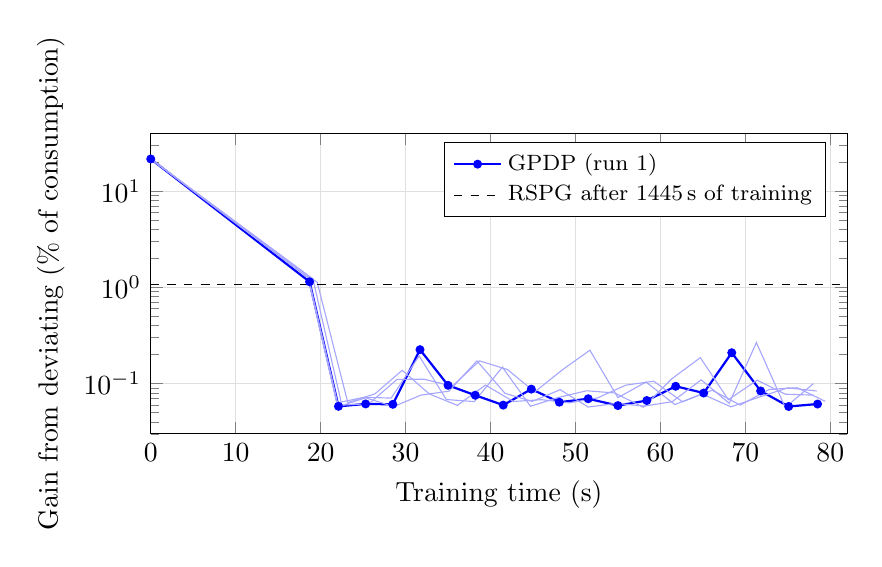
\begin{tikzpicture}
\begin{axis}[
  width=0.86\linewidth, height=5.4cm,
  xlabel={Training time (s)}, ylabel={Gain from deviating (\% of consumption)},
  ymode=log, ymin=0.03, ymax=40, xmin=0, xmax=82,
  legend pos=north east, legend cell align=left, legend style={font=\footnotesize},
  grid=major, grid style={gray!25}]
\addplot[blue, thick, mark=*, mark size=1.2pt] coordinates {(0.0,21.57) (18.7,1.141) (22.1,0.05791) (25.3,0.06136) (28.5,0.06077) (31.7,0.2249) (35.0,0.09584) (38.2,0.07552) (41.5,0.05961) (44.8,0.08744) (48.1,0.06391) (51.5,0.06944) (55.0,0.05895) (58.4,0.06654) (61.8,0.0936) (65.1,0.07967) (68.4,0.2088) (71.8,0.08366) (75.1,0.0577) (78.5,0.0612)};
\addlegendentry{GPDP (run 1)}
\addplot[blue!35, thin, forget plot] coordinates {(0.0,21.57) (18.5,1.271) (21.9,0.06274) (25.1,0.07193) (28.3,0.07054) (31.6,0.1933) (34.8,0.06817) (38.1,0.06485) (41.4,0.1479) (44.7,0.05804) (48.0,0.07166) (51.3,0.08403) (54.6,0.07981) (58.0,0.05663) (61.3,0.1113) (64.7,0.1856) (68.0,0.06789) (71.4,0.1084) (74.7,0.07744) (78.1,0.07567)};
\addplot[blue!35, thin, forget plot] coordinates {(0.0,21.57) (18.6,1.24) (22.1,0.0575) (25.3,0.07101) (28.6,0.05761) (31.8,0.0757) (35.1,0.08328) (38.4,0.1717) (41.7,0.07911) (44.9,0.06513) (48.2,0.08618) (51.5,0.05694) (54.8,0.06212) (58.1,0.05824) (61.4,0.06477) (64.8,0.1092) (68.1,0.06234) (71.3,0.2663) (74.7,0.05633) (78.0,0.09969)};
\addplot[blue!35, thin, forget plot] coordinates {(0.0,21.57) (19.1,1.217) (22.5,0.05963) (25.7,0.06169) (29.0,0.1105) (32.2,0.1107) (35.5,0.09389) (38.7,0.172) (42.0,0.1397) (45.2,0.08166) (48.5,0.1396) (51.7,0.2221) (55.0,0.07124) (58.3,0.1036) (61.7,0.06043) (64.9,0.07802) (68.3,0.0572) (71.7,0.07256) (75.0,0.09018) (78.4,0.08356)};
\addplot[blue!35, thin, forget plot] coordinates {(0.0,21.57) (19.6,1.126) (23.2,0.06334) (26.4,0.07812) (29.6,0.1372) (32.8,0.07786) (36.1,0.05926) (39.4,0.0963) (42.7,0.06504) (46.0,0.06792) (49.3,0.06299) (52.6,0.07088) (55.9,0.09598) (59.2,0.1057) (62.6,0.0646) (66.1,0.08521) (69.4,0.05964) (72.8,0.08677) (76.1,0.09037) (79.4,0.06529)};
\addplot[black, dashed, domain=0:82] {1.06};
\addlegendentry{RSPG after 1445\,s of training}
\end{axis}
\end{tikzpicture}
\caption{Gain from deviating during GPDP training (5 runs, run 1 highlighted), measured on 32
monitoring economies against a best response allowed any share. Each point is placed at the time its
decision rule was produced. The dashed line is RSPG's value at the end of its training.}
\label{fig:conv}
\end{figure}

\begin{itemize}
\item \textbf{Speed.} GPDP reaches the equilibrium after 2 iterations, about 22\,s of training (10\,s
  without the one-off compilation), against about 1080\,s for RSPG. One GPDP iteration costs about
  as much as one RSPG step; GPDP needs 2 of them where RSPG needs hundreds.
\item \textbf{Accuracy on MFAX's own metric.} GPDP's exploitability is about 30\% lower than
  RSPG's, although GPDP is trained with continuous shares and only mapped to MFAX's 20 shares for
  this evaluation.
\item \textbf{Accuracy in consumption units.} Against a best response allowed any share, a household
  gains 0.09\% of consumption by deviating from GPDP, against 1.06\% from RSPG. Most of RSPG's gap
  comes from its 20-share grid: in RSPG's economy, choosing shares freely is worth about 1.3\% of
  consumption on average.
\item \textbf{Stability.} After converging, the gain stays between 0.06\% and 0.27\% from one
  iteration to the next (Figure~\ref{fig:conv}): the population adopts each new rule in full and the
  value GP is refitted every iteration. A lower bound of about 0.06\% is expected: the best response
  used here knows the realized shocks, which no household can.
\end{itemize}

\begin{table}[h]
\centering
\small
\caption{CE relative error by period of the episode (\% of consumption, population-weighted).}
\label{tab:blocks}
\begin{tabular}{lcccccc}
\toprule
Periods & 0--31 & 32--63 & 64--95 & 96--111 & 112--119 & 120--126 \\
\midrule
RSPG          & 1.7 & 2.3 & 5.2 & 14.6 & 29.4 & 50.4 \\
\textbf{GPDP} & \textbf{0.06} & \textbf{0.05} & \textbf{0.04} & \textbf{0.03} & \textbf{0.02} & \textbf{0.01} \\
\bottomrule
\end{tabular}
\end{table}

Table~\ref{tab:blocks} shows where in the episode the errors are (both methods against a best
response allowed any share; 5 runs each). RSPG is accurate early but its error grows to 50\% in the
last periods: with a known end date, a household should spend its savings as the end approaches,
and RSPG's rule barely does. Exploitability hardly sees this, because it discounts everything back
to period 0 ($\gamma^{120} \approx 0.002$). GPDP stays accurate in every period: its households raise
their consumption share from 0.13 in mid-episode to 0.22 at period 120 and 0.58 at period 126, and
capital falls from 27.8 at period 100 to 2.9 at period 127, as the finite horizon requires.

%=====================================================================
\section{Limitations}
\begin{itemize}
\item \textbf{The decision rule needs the time left as an input.} Without it, the policy GP cannot
  represent the best decisions, which change strongly near the end of the episode, and the iteration
  does not settle; replacing it by RSPG's learned memory of prices did not help. RSPG, by contrast,
  works without an explicit date.
\item \textbf{One model.} Here the economy is well summarized by $(z, K)$, prices reveal it, and
  aggregate shocks are small. A model where prices do not reveal the state is the natural next test.
\item \textbf{Robustness.} The GP fits need bounded hyperparameters to stay numerically stable. All 5
  runs reported here converged; in earlier variants of the implementation, one run in five failed
  numerically.
\item \textbf{Hardware.} Timings are on a laptop CPU; on a GPU, RSPG's long simulations parallelize
  better.
\end{itemize}

%=====================================================================
\section{Extension: a learned law of motion}\label{sec:lom}

\subsection{The idea in GPDP}

The implementation above uses the model's dynamics directly: tomorrow's capital $K_{t+1}^n$ is read
off the simulated distribution $\mu_{t+1}^n$. The GPDP paper~\cite{deisenroth} does not assume the
dynamics are known (its Section~4). It learns them with a GP from observed transitions
$x_t \mapsto x_{t+1} - x_t$, which gives a Gaussian prediction of the next state, and then averages
the value GP over that uncertain next state \emph{in closed form} (its Appendix~A). The data that
train the dynamics GP and the states at which values are computed (the support points) can be
chosen separately. In reinforcement-learning terms, the dynamics GP is a learned \emph{world model}.
This section tests whether this part of GPDP works in our game.

The closed form rests on one result. For a GP $\widehat f$ with a squared-exponential kernel and an
input that is Gaussian, $x' \sim \mathcal N(m, S)$, the expected prediction is exact:
\[
\mathbb E\big[\widehat f(x')\big] = \bar y + \sigma_y \sum_{i} \beta_i\, l_i, \qquad
l_i = s_f^2\, \big|S\Lambda^{-1} + I\big|^{-1/2}
\exp\!\Big(-\tfrac12 (x_i - m)^\top (S + \Lambda)^{-1} (x_i - m)\Big),
\]
where $x_i$ are the GP's training inputs, $\beta = (K + s_n^2 I)^{-1} y$ its weights,
$\Lambda = \mathrm{diag}(\ell_1^2, \ell_2^2, \ell_3^2)$, all in standardized units, and $\bar y$,
$\sigma_y$ undo the output standardization. Only the \emph{input} must be Gaussian; the outputs can
have any distribution.

\subsection{Our implementation}

\paragraph{The law-of-motion GP.} In our game the part of the dynamics that a household must forecast
is aggregate capital: the shock follows a known AR(1), and the household's own transition is known
exactly. A third GP therefore predicts the change in capital from the state of the economy,
\[
x = (z_t, K_t, \tau) \;\longmapsto\; K_{t+1} - K_t ,
\]
trained on the $8 \times 127$ transitions of each forward pass. The household's action is not an
input: a single household does not move capital. This is a learned version of Krusell and Smith's
``perceived law of motion''~\cite{ks}, the rule households use to forecast capital. Its prediction
is Gaussian, $K_{t+1} \sim \mathcal N\big(K_t + m(x),\, s^2(x)\big)$, where $s^2$ includes the GP's
noise term: the part of $K_{t+1}$ that $(z, K, \tau)$ does not determine.

\paragraph{Tomorrow's input is Gaussian.} Tomorrow's capital comes from the law of motion,
tomorrow's shock is Gaussian, and the time left drops by one. So tomorrow's input to the value GP is
\[
x' = (z', K', \tau - 1) \;\sim\; \mathcal N\Big(\big(0.9\,z_t,\; K_t + m(x),\; \tau - 1\big),\;
\mathrm{diag}\big(0.03^2,\; s^2(x),\; 0\big)\Big),
\]
and the closed form above gives tomorrow's expected value. It replaces both the 5 quadrature points
over $z'$ and the exact $K_{t+1}$ of Section~\ref{sec:backward}. One vector $l$ serves all 1000
household states.

\paragraph{From $\log \bar c$ to values.} Our value GP predicts $y = \log \bar c$, and the value
$V = D(\tau)\,u(e^{y})$ is a curved function of it, so $\mathbb E[V] \neq D(\tau)\,u\big(e^{\mathbb E[y]}\big)$.
We use the lognormal moment,
$\mathbb E[V] = D(\tau)\, u\big(e^{\mathbb E[y]}\big)\, e^{(1-\sigma)^2 \mathrm{Var}[y]/2}$, with
$\mathbb E[y]$ from the closed form and $\mathrm{Var}[y]$ from a first-order expansion of the GP
around $m$. In the last decision period the continuation is the known terminal utility, not a GP;
there we keep quadrature, now over both $z'$ and $K'$ ($5 \times 5$ points).

\paragraph{Where the backward pass is solved.} A household's utility and next state depend on the
economy only through the prices and the date, and the prices are a function of $(z, K)$. With the law
of motion, the backward pass therefore needs only $(z, K, \tau)$ at each support point, not the
distribution $\mu$. We test two choices of support points:
\begin{enumerate}[label=(\alph*)]
\item \textbf{The simulated economies.} Today's $(z_t, K_t)$ come from the simulation, as before;
  only tomorrow's capital is forecast by the law of motion. Each forecast starts from a true state.
\item \textbf{Paths simulated by the law of motion itself.} 8 paths start from the initial state;
  $z$ follows its AR(1), and $K$ follows the GP's forecast plus its noise. Today's $K_t$ is then the
  GP's own previous forecast, so forecast errors carry over from one period to the next. The
  simulated distributions are used only to train the law of motion.
\end{enumerate}
For example, if the simulation gives $K_{50} = 25.00$ and $K_{51} = 25.31$, and the GP forecasts
$25.29$ from $K_{50}$: in (a) the support point at period 51 has $K = 25.31$; in (b) it has
$K = 25.29$, and the next forecast starts from there.

\paragraph{What it took.} Three choices were needed for the law of motion to be accurate:
\begin{itemize}
\item \textbf{Double precision.} Its targets are almost noiseless. In single precision the
  hyperparameter fit failed on its first steps, and the predictive variance, a difference of two
  nearly equal numbers, was lost to rounding.
\item \textbf{$\log \tau$ as input instead of $\tau$.} Capital falls steeply in the last periods,
  as households spend their savings. On the log scale the end of the episode gets the resolution it
  needs.
\item \textbf{A fresh fit every iteration.} Starting the hyperparameters from the previous
  iteration's got stuck: the first iteration's constant 15\% share has no end-of-episode fall in
  capital, so the fitted time length scale was very long, and later fits did not recover.
\end{itemize}

\subsection{Metrics and results}

\paragraph{Metrics.} The decision rules are evaluated exactly as in Section~\ref{sec:metrics}:
exploitability, CE relative error and training time to converge, on the same 64 evaluation
economies. The law of motion itself is measured on economies it was not trained on, by
\begin{itemize}
\item the $R^2$ of its prediction of $K_{t+1} - K_t$ (the share of the variation in the change of
  capital that it explains);
\item its largest relative error, $\max |\widehat K_{t+1} - K_{t+1}| / K_{t+1}$ over all transitions;
\item its calibration: how often the realized $K_{t+1}$ falls inside its predicted 95\% band.
\end{itemize}

\paragraph{Checks.} Table~\ref{tab:lomchecks} tests each piece separately, against the final decision
rule of one GPDP run.

\begin{table}[h]
\centering
\small
\caption{Checks of the law of motion and the closed form (law of motion trained on 8 simulated
economies, tested on 64 new ones).}
\label{tab:lomchecks}
\begin{tabularx}{\linewidth}{@{}>{\raggedright\arraybackslash}X>{\raggedright\arraybackslash}p{6.3cm}@{}}
\toprule
Check & Result \\
\midrule
Law of motion: $R^2$ of $K_{t+1} - K_t$ & 0.999996; largest error 0.08\% of $K_{t+1}$ \\
Krusell--Smith log-linear rule ($\log K'$ on $\log K$, $z$, $\tau$), same data & $R^2$ of $K_{t+1} - K_t$: $-0.32$ \\
Calibration: realized $K_{t+1}$ inside the predicted 95\% band & 89\% of transitions \\
Closed form vs 40-point quadrature, $K_{t+1}$ exact & at most 0.015\% of $V$ (5-point quadrature: 0.016\%) \\
\quad the same without the lognormal correction & at most 0.049\% \\
Closed form vs Monte Carlo (20{,}000 draws), $K_{t+1}$ uncertain & at most 0.026\% \\
Backward pass with law of motion vs exact $K_{t+1}$ & best shares differ by 0.0001 on average;
values by 0.002\% (CE) \\
\bottomrule
\end{tabularx}
\end{table}

The Krusell--Smith rule fails here because a single log-linear rule cannot follow both the build-up
of capital from the uniform start and its fall at the end of the episode; the GP can.

\paragraph{Results.} Both variants were trained exactly as in Section~\ref{sec:results} (5 runs,
20 iterations, the same 64 evaluation economies). Table~\ref{tab:lom} compares them with the
implementation of Section~\ref{sec:impl}.

\begin{table}[h]
\centering
\small
\caption{GPDP with a learned law of motion (mean $\pm$ standard deviation over 5 runs).}
\label{tab:lom}
\begin{tabularx}{\linewidth}{@{}>{\raggedright\arraybackslash}Xccc@{}}
\toprule
 & $K_{t+1}$ from the & (a) law of motion, & (b) law of motion, \\
 & simulation (Sec.~\ref{sec:impl}) & simulated economies & its own paths \\
\midrule
Exploitability (MFAX)                   & $0.027 \pm 0.008$ & $0.027 \pm 0.008$ & $0.027 \pm 0.003$ \\
Gain from deviating (\% of consumption) & 0.09\%  & 0.09\%  & 0.09\% \\
CE relative error, start of episode     & 0.08\%  & 0.08\%  & 0.08\% \\
CE relative error, all periods          & 0.044\% & 0.044\% & 0.044\% \\
Iterations to converge                  & 2       & 2       & 2 \\
Training time to converge               & 22 s    & 32 s    & 32 s \\
Time per iteration                      & 3.3 s   & 7.8 s   & 7.9 s \\
Law of motion: largest error on the evaluation economies & -- & 0.11\% & 0.11\% \\
\bottomrule
\end{tabularx}

\smallskip
\begin{minipage}{0.92\linewidth}\footnotesize
Last row: largest error of the predicted $K_{t+1}$ over all transitions of the 32 monitoring
economies, median over iterations 2--19 and runs. In 2 of the 90 iterations of variant (a), the
hyperparameter fit was poorer (largest error 2.0\% and 7.4\%), without visible effect on the gain.
\end{minipage}
\end{table}

\begin{itemize}
\item \textbf{It works.} With the learned law of motion and the closed-form expectation, GPDP
  reaches the same accuracy as with the simulated capital, on every metric, in the same 2
  iterations. This holds even in variant (b), where the backward pass never sees a simulated
  distribution: the law of motion's 127-step paths stay close enough to real ones.
\item \textbf{What it changes.} The backward pass needs only $(z, K, \tau)$, and tomorrow's
  uncertainty (shock and capital) is averaged in one closed-form step, the same for all 1000
  household states.
\item \textbf{Cost.} About 4.5\,s more per iteration, almost all of it the law of motion's own
  hyperparameter fit (300 steps in double precision on 1016 points: 4.4\,s). With 100 steps the
  fit takes 1.7\,s and is about as accurate (largest error 0.16\% vs 0.18\%, one check), but the
  runs above used 300.
\item \textbf{Numerics.} Single precision was the source of every failure met here. In one
  iteration out of 100 in variant (b), the policy GP's factorization failed in single precision; the
  previous decision rule was then kept for one iteration. Fitting all GPs in double precision is a
  natural next step.
\end{itemize}

\begin{thebibliography}{9}
\bibitem{aiyagari}
S.~R. Aiyagari. Uninsured idiosyncratic risk and aggregate saving.
\emph{Quarterly Journal of Economics}, 109(3):659--684, 1994.
\bibitem{deisenroth}
M.~P. Deisenroth, C.~E. Rasmussen, and J.~Peters.
Gaussian process dynamic programming.
\emph{Neurocomputing}, 72(7--9):1508--1524, 2009.
\bibitem{ks}
P.~Krusell and A.~A. Smith.
Income and wealth heterogeneity in the macroeconomy.
\emph{Journal of Political Economy}, 106(5):867--896, 1998.
\bibitem{rspg}
C.~Wibault et al.
Recurrent structural policy gradient for partially observable mean field games.
2026. \href{https://arxiv.org/abs/2602.20141}{arXiv:2602.20141}.
\bibitem{spg}
Y.~Yang, C.~Wang, A.~Schaab, and B.~Moll.
Structural reinforcement learning for heterogeneous agent macroeconomics.
2025. \href{https://arxiv.org/abs/2512.18892}{arXiv:2512.18892}.
\end{thebibliography}

\end{document}
